\documentclass{article}
\usepackage{tikz}

\begin{document}

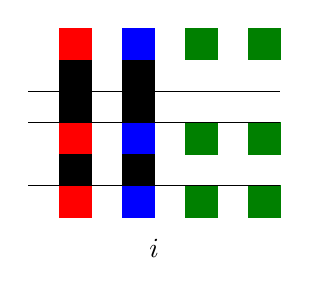
\begin{tikzpicture}[scale=0.8]
    % Define colors
    \definecolor{black}{RGB}{0,0,0}
    \definecolor{red}{RGB}{255,0,0}
    \definecolor{blue}{RGB}{0,0,255}
    \definecolor{green}{RGB}{0,128,0}

    % Draw the first row of boxes
    \foreach \x in {0,1} {
        \filldraw[black] (\x,0) rectangle ++(0.5,0.5);
    }
    \foreach \x in {0,1} {
        \filldraw[red] (0+\x,0.5) rectangle ++(0.5,0.5);
    }
    \foreach \x in {0,1} {
        \filldraw[blue] (1+\x,0.5) rectangle ++(0.5,0.5);
    }
    \foreach \x in {0,1} {
        \filldraw[green] (2+\x,0.5) rectangle ++(0.5,0.5);
    }

    % Draw the second row of boxes
    \foreach \x in {0,1} {
        \filldraw[black] (\x,-0.5) rectangle ++(0.5,0.5);
    }
    \foreach \x in {0,1} {
        \filldraw[red] (0+\x,-1) rectangle ++(0.5,0.5);
    }
    \foreach \x in {0,1} {
        \filldraw[blue] (1+\x,-1) rectangle ++(0.5,0.5);
    }
    \foreach \x in {0,1} {
        \filldraw[green] (2+\x,-1) rectangle ++(0.5,0.5);
    }

    % Draw the third row of boxes
    \foreach \x in {0,1} {
        \filldraw[black] (\x,-1.5) rectangle ++(0.5,0.5);
    }
    \foreach \x in {0,1} {
        \filldraw[red] (0+\x,-2) rectangle ++(0.5,0.5);
    }
    \foreach \x in {0,1} {
        \filldraw[blue] (1+\x,-2) rectangle ++(0.5,0.5);
    }
    \foreach \x in {0,1} {
        \filldraw[green] (2+\x,-2) rectangle ++(0.5,0.5);
    }

    % Draw the horizontal line
    \draw (-0.5,0) -- (3.5,0);
    \draw (-0.5,-0.5) -- (3.5,-0.5);
    \draw (-0.5,-1.5) -- (3.5,-1.5);

    % Label the row index
    \node at (1.5,-2.5) {$i$};
\end{tikzpicture}

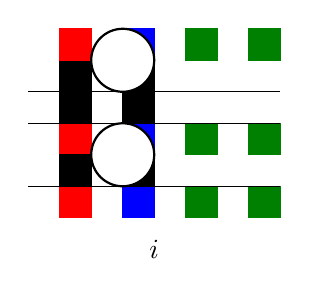
\begin{tikzpicture}[scale=0.8]
    % Define colors
    \definecolor{black}{RGB}{0,0,0}
    \definecolor{red}{RGB}{255,0,0}
    \definecolor{blue}{RGB}{0,0,255}
    \definecolor{green}{RGB}{0,128,0}

    % Draw the first row of boxes
    \foreach \x in {0,1} {
        \filldraw[black] (\x,0) rectangle ++(0.5,0.5);
    }
    \foreach \x in {0,1} {
        \filldraw[red] (0+\x,0.5) rectangle ++(0.5,0.5);
    }
    \foreach \x in {0,1} {
        \filldraw[blue] (1+\x,0.5) rectangle ++(0.5,0.5);
    }
    \foreach \x in {0,1} {
        \filldraw[green] (2+\x,0.5) rectangle ++(0.5,0.5);
    }

    % Draw the second row of boxes
    \foreach \x in {0,1} {
        \filldraw[black] (\x,-0.5) rectangle ++(0.5,0.5);
    }
    \foreach \x in {0,1} {
        \filldraw[red] (0+\x,-1) rectangle ++(0.5,0.5);
    }
    \foreach \x in {0,1} {
        \filldraw[blue] (1+\x,-1) rectangle ++(0.5,0.5);
    }
    \foreach \x in {0,1} {
        \filldraw[green] (2+\x,-1) rectangle ++(0.5,0.5);
    }

    % Draw the third row of boxes
    \foreach \x in {0,1} {
        \filldraw[black] (\x,-1.5) rectangle ++(0.5,0.5);
    }
    \foreach \x in {0,1} {
        \filldraw[red] (0+\x,-2) rectangle ++(0.5,0.5);
    }
    \foreach \x in {0,1} {
        \filldraw[blue] (1+\x,-2) rectangle ++(0.5,0.5);
    }
    \foreach \x in {0,1} {
        \filldraw[green] (2+\x,-2) rectangle ++(0.5,0.5);
    }

    % Draw the horizontal line
    \draw (-0.5,0) -- (3.5,0);
    \draw (-0.5,-0.5) -- (3.5,-0.5);
    \draw (-0.5,-1.5) -- (3.5,-1.5);

    % Draw the circle around the middle row
    \draw[thick, black, fill=white] (1,0.5) circle (0.5);
    \draw[thick, black, fill=white] (1,-1) circle (0.5);

    % Label the row index
    \node at (1.5,-2.5) {$i$};
\end{tikzpicture}

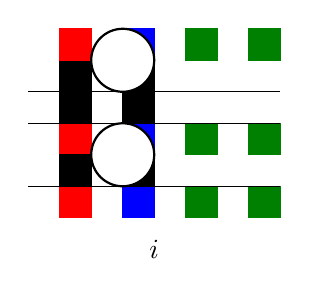
\begin{tikzpicture}[scale=0.8]
    % Define colors
    \definecolor{black}{RGB}{0,0,0}
    \definecolor{red}{RGB}{255,0,0}
    \definecolor{blue}{RGB}{0,0,255}
    \definecolor{green}{RGB}{0,128,0}

    % Draw the first row of boxes
    \foreach \x in {0,1} {
        \filldraw[black] (\x,0) rectangle ++(0.5,0.5);
    }
    \foreach \x in {0,1} {
        \filldraw[red] (0+\x,0.5) rectangle ++(0.5,0.5);
    }
    \foreach \x in {0,1} {
        \filldraw[blue] (1+\x,0.5) rectangle ++(0.5,0.5);
    }
    \foreach \x in {0,1} {
        \filldraw[green] (2+\x,0.5) rectangle ++(0.5,0.5);
    }

    % Draw the second row of boxes
    \foreach \x in {0,1} {
        \filldraw[black] (\x,-0.5) rectangle ++(0.5,0.5);
    }
    \foreach \x in {0,1} {
        \filldraw[red] (0+\x,-1) rectangle ++(0.5,0.5);
    }
    \foreach \x in {0,1} {
        \filldraw[blue] (1+\x,-1) rectangle ++(0.5,0.5);
    }
    \foreach \x in {0,1} {
        \filldraw[green] (2+\x,-1) rectangle ++(0.5,0.5);
    }

    % Draw the third row of boxes
    \foreach \x in {0,1} {
        \filldraw[black] (\x,-1.5) rectangle ++(0.5,0.5);
    }
    \foreach \x in {0,1} {
        \filldraw[red] (0+\x,-2) rectangle ++(0.5,0.5);
    }
    \foreach \x in {0,1} {
        \filldraw[blue] (1+\x,-2) rectangle ++(0.5,0.5);
    }
    \foreach \x in {0,1} {
        \filldraw[green] (2+\x,-2) rectangle ++(0.5,0.5);
    }

    % Draw the horizontal line
    \draw (-0.5,0) -- (3.5,0);
    \draw (-0.5,-0.5) -- (3.5,-0.5);
    \draw (-0.5,-1.5) -- (3.5,-1.5);

    % Draw the circle around the middle row
    \draw[thick, black, fill=white] (1,0.5) circle (0.5);
    \draw[thick, black, fill=white] (1,-1) circle (0.5);

    % Label the row index
    \node at (1.5,-2.5) {$i$};
\end{tikzpicture}

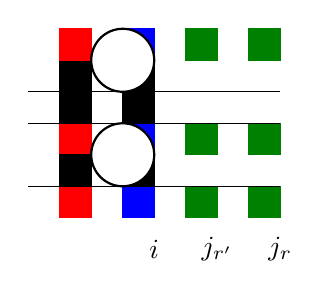
\begin{tikzpicture}[scale=0.8]
    % Define colors
    \definecolor{black}{RGB}{0,0,0}
    \definecolor{red}{RGB}{255,0,0}
    \definecolor{blue}{RGB}{0,0,255}
    \definecolor{green}{RGB}{0,128,0}

    % Draw the first row of boxes
    \foreach \x in {0,1} {
        \filldraw[black] (\x,0) rectangle ++(0.5,0.5);
    }
    \foreach \x in {0,1} {
        \filldraw[red] (0+\x,0.5) rectangle ++(0.5,0.5);
    }
    \foreach \x in {0,1} {
        \filldraw[blue] (1+\x,0.5) rectangle ++(0.5,0.5);
    }
    \foreach \x in {0,1} {
        \filldraw[green] (2+\x,0.5) rectangle ++(0.5,0.5);
    }

    % Draw the second row of boxes
    \foreach \x in {0,1} {
        \filldraw[black] (\x,-0.5) rectangle ++(0.5,0.5);
    }
    \foreach \x in {0,1} {
        \filldraw[red] (0+\x,-1) rectangle ++(0.5,0.5);
    }
    \foreach \x in {0,1} {
        \filldraw[blue] (1+\x,-1) rectangle ++(0.5,0.5);
    }
    \foreach \x in {0,1} {
        \filldraw[green] (2+\x,-1) rectangle ++(0.5,0.5);
    }

    % Draw the third row of boxes
    \foreach \x in {0,1} {
        \filldraw[black] (\x,-1.5) rectangle ++(0.5,0.5);
    }
    \foreach \x in {0,1} {
        \filldraw[red] (0+\x,-2) rectangle ++(0.5,0.5);
    }
    \foreach \x in {0,1} {
        \filldraw[blue] (1+\x,-2) rectangle ++(0.5,0.5);
    }
    \foreach \x in {0,1} {
        \filldraw[green] (2+\x,-2) rectangle ++(0.5,0.5);
    }

    % Draw the horizontal line
    \draw (-0.5,0) -- (3.5,0);
    \draw (-0.5,-0.5) -- (3.5,-0.5);
    \draw (-0.5,-1.5) -- (3.5,-1.5);

    % Draw the circle around the middle row
    \draw[thick, black, fill=white] (1,0.5) circle (0.5);
    \draw[thick, black, fill=white] (1,-1) circle (0.5);

    % Label the row indices
    \node at (1.5,-2.5) {$i$};
    \node at (2.5,-2.5) {$j_{r'}$};
    \node at (3.5,-2.5) {$j_r$};
\end{tikzpicture}

\end{document}